\documentclass[UTF8]{ctexart}
\usepackage{tikz}
\usepackage[top=1in, bottom=1in, left=0.5in, right=1.25in]{geometry}
\usepackage{amsmath}
\usetikzlibrary{shapes}
\geometry{papersize={21.59cm,137.94cm}}
\begin{document}
\begin{large}
\noindent
数组(minimum degree t=2):
$
 \begin{mathcal}
[F , S , Q , K , C , L , H , T , V , W , M , R , N , P , A , B , X , Y , D , Z , E]
 \end{mathcal}$
\\

\begin{enumerate}
\item 插入F


\begin{center}

\begin{tikzpicture}
\tikzstyle{bplus}=[rectangle split, rectangle split horizontal,black,fill=gray!10,rectangle split ignore empty parts,draw]
\tikzstyle{every node}=[bplus]
\node[bplus] at (0,0) {. \nodepart{two} F  \nodepart{three} .};
\end{tikzpicture}
\newline
\end{center}


\item 插入S


\begin{center}
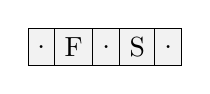
\begin{tikzpicture}
\tikzstyle{bplus}=[rectangle split, rectangle split horizontal,rectangle split parts=#1,black,fill=gray!10,rectangle split ignore empty parts,draw]
\tikzstyle{every node}=[bplus]
\node[bplus=5] at (0,0) {. \nodepart{two} F \nodepart{three} .  \nodepart{four} S  \nodepart{five} .  };
\end{tikzpicture}
\newline
\end{center}



\item 插入Q


\begin{center}
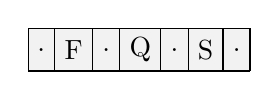
\begin{tikzpicture}
\tikzstyle{bplus}=[rectangle split, rectangle split horizontal,rectangle split parts=#1,black,fill=gray!10,rectangle split ignore empty parts,draw]
\tikzstyle{every node}=[bplus]
\node[bplus=8] at (0,0) { . \nodepart{two}  F \nodepart{three} . \nodepart{four}  Q \nodepart{five} . \nodepart{six}  S  \nodepart{seven}. };
\end{tikzpicture}
\newline
\end{center}



\item 插入K ($ [F,Q,S].length \geq 2 \times t = 3 ,split [F,Q,S] $)


\begin{center}
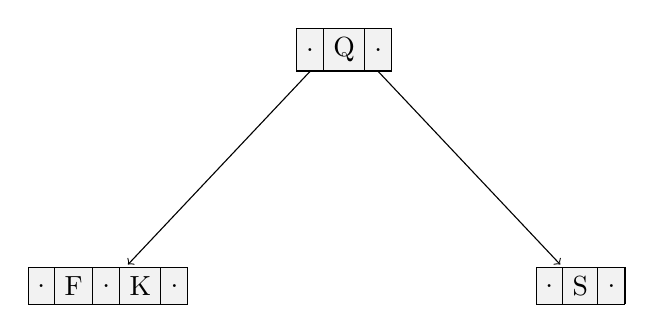
\begin{tikzpicture}[shorten >=1pt,node distance=12cm,auto]
\tikzstyle{bplus}=[rectangle split, rectangle split horizontal,rectangle split parts=#1,black,fill=gray!10,rectangle split ignore empty parts,draw]
\tikzstyle{every node}=[bplus]
\node[bplus](Q) at (3,3) { . \nodepart{two} Q  \nodepart{three} .};
\node[bplus=5](F) at (0,0) { . \nodepart{two} F  \nodepart{three} . \nodepart{four}  K \nodepart{five} . };
\node[bplus](S) at (6,0) {. \nodepart{two} S  \nodepart{three} .};

\path (Q.one south) edge[->] (F) % simple edges
      (Q.three south) edge[->] (S);

\end{tikzpicture}
\newline
% \newpage
\end{center}



\item 插入C


\begin{center}
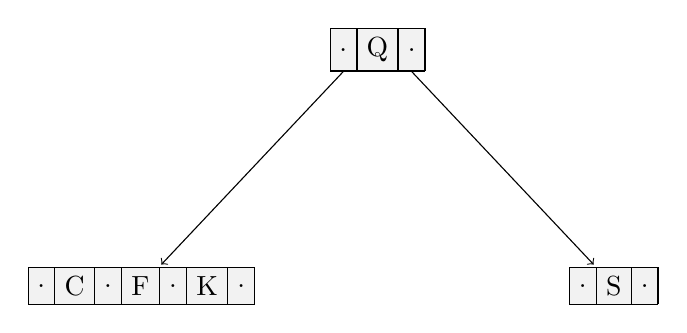
\begin{tikzpicture}[shorten >=1pt,node distance=12cm,auto]
\tikzstyle{bplus}=[rectangle split, rectangle split horizontal,rectangle split parts=#1,black,fill=gray!10,rectangle split ignore empty parts,draw]
\tikzstyle{every node}=[bplus]
\node[bplus](Q) at (3,3) { . \nodepart{two} Q  \nodepart{three} .};
\node[bplus=7](F) at (0,0) { . \nodepart{two} C   \nodepart{three} .  \nodepart{four} F \nodepart{five}  . \nodepart{six} K \nodepart{seven} .};
\node[bplus](S) at (6,0) {. \nodepart{two} S  \nodepart{three} .};

\path (Q.one south) edge[->] (F) % simple edges
      (Q.three south) edge[->] (S);

\end{tikzpicture}
\newline
\end{center}


\item 插入L ($ [C,F,K].length \geq 2 \times t = 3  ,split [C,F,K] $)


\begin{center}
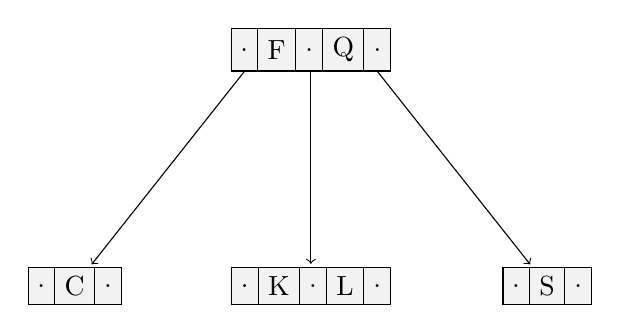
\begin{tikzpicture}[shorten >=1pt,node distance=12cm,auto]
\tikzstyle{bplus}=[rectangle split, rectangle split horizontal,rectangle split parts=#1,black,fill=gray!10,rectangle split ignore empty parts,draw]
\tikzstyle{every node}=[bplus]
\node[bplus=5](Q) at (3,3) { . \nodepart{two}  F  \nodepart{three} . \nodepart{four} Q   \nodepart{five}.};
\node[bplus](C) at (0,0) { . \nodepart{two} C   \nodepart{three} .};
\node[bplus=5](K) at (3,0) {. \nodepart{two} K \nodepart{three}. \nodepart{four} L \nodepart{five} . };
\node[bplus](S) at (6,0) {. \nodepart{two} S  \nodepart{three} .};


\draw[->] (Q.one south) -> (C);
\draw[->] (Q) -> (K);
\draw[->] (Q.five south) -> (S);
\end{tikzpicture}
\newline
\end{center}


\item 插入H

\begin{center}
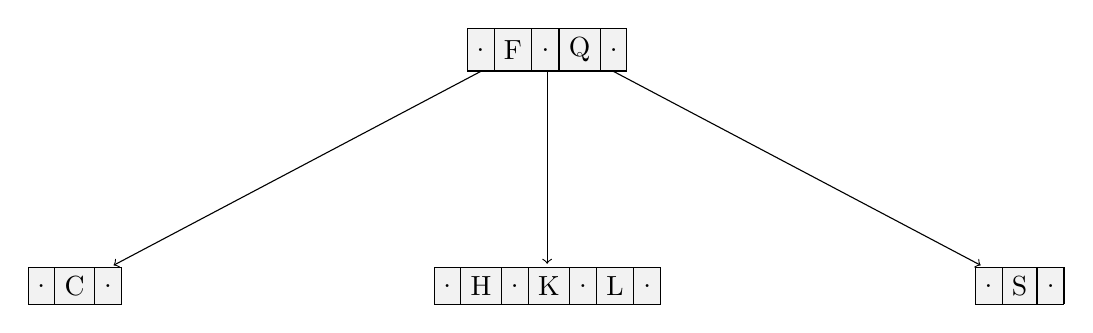
\begin{tikzpicture}[shorten >=1pt,node distance=12cm,auto]
\tikzstyle{bplus}=[rectangle split, rectangle split horizontal,rectangle split parts=#1,black,fill=gray!10,rectangle split ignore empty parts,draw]
\tikzstyle{every node}=[bplus]
\node[bplus=5](Q) at (6,3) { . \nodepart{two}  F  \nodepart{three} . \nodepart{four} Q   \nodepart{five}.};
\node[bplus](C) at (0,0) { . \nodepart{two} C   \nodepart{three} .};
\node[bplus=7](K) at (6,0) {. \nodepart{two} H \nodepart{three} . \nodepart{four} K \nodepart{five} . \nodepart{six} L \nodepart{seven} .};
\node[bplus](S) at (12,0) {. \nodepart{two} S  \nodepart{three} .};


\draw[->] (Q.one south) -> (C);
\draw[->] (Q) -> (K);
\draw[->] (Q.five south) -> (S);
\end{tikzpicture}
\newline
\end{center}


\item 插入T

\begin{center}
\begin{tikzpicture}[shorten >=1pt,node distance=12cm,auto]
\tikzstyle{bplus}=[rectangle split, rectangle split horizontal,rectangle split parts=#1,black,fill=gray!10,rectangle split ignore empty parts,draw]
\tikzstyle{every node}=[bplus]
\node[bplus=5](Q) at (6,3) { . \nodepart{two}  F  \nodepart{three} . \nodepart{four} Q   \nodepart{five}.};
\node[bplus](C) at (0,0) { . \nodepart{two} C   \nodepart{three} .};
\node[bplus=7](K) at (6,0) {. \nodepart{two} H \nodepart{three} . \nodepart{four} K \nodepart{five} . \nodepart{six} L \nodepart{seven} .};
\node[bplus](S=5) at (12,0) {. \nodepart{two} S   \nodepart{three} . \nodepart{four} T \nodepart{five} .};



\draw[->] (Q.one south) -> (C);
\draw[->] (Q) -> (K);
\draw[->] (Q.five south) -> (S);
\end{tikzpicture}
\newline
\end{center}


\item 插入V

\begin{center}
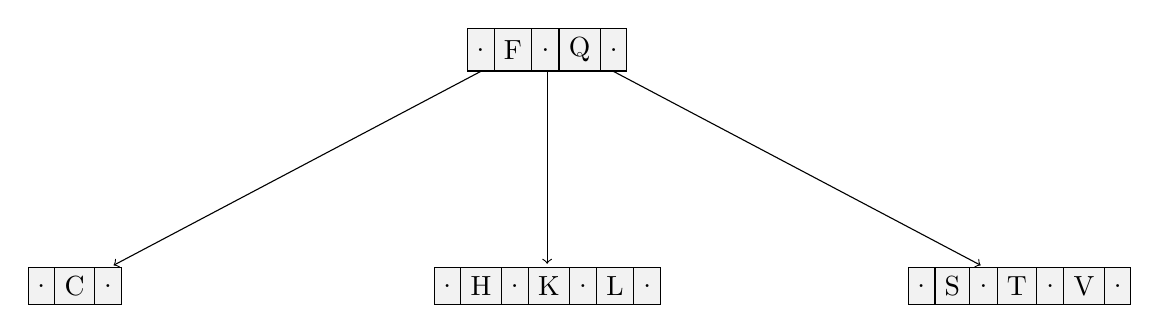
\begin{tikzpicture}[shorten >=1pt,node distance=12cm,auto]
\tikzstyle{bplus}=[rectangle split, rectangle split horizontal,rectangle split parts=#1,black,fill=gray!10,rectangle split ignore empty parts,draw]
\tikzstyle{every node}=[bplus]
\node[bplus=5](Q) at (6,3) { . \nodepart{two}  F  \nodepart{three} . \nodepart{four} Q   \nodepart{five}.};
\node[bplus](C) at (0,0) { . \nodepart{two} C   \nodepart{three} .};
\node[bplus=7](K) at (6,0) {. \nodepart{two} H \nodepart{three} . \nodepart{four} K \nodepart{five} . \nodepart{six} L \nodepart{seven} .};
\node[bplus=7](S) at (12,0) {. \nodepart{two} S   \nodepart{three} . \nodepart{four} T \nodepart{five} . \nodepart{six} V \nodepart{seven} .};



\draw[->] (Q.one south) -> (C);
\draw[->] (Q) -> (K);
\draw[->] (Q.five south) -> (S);
\end{tikzpicture}
\newline
\end{center}


\item 插入W ($ [S,T,V].length \geq 2 \times t = 3  ,split [S,T,V] $)

\begin{center}
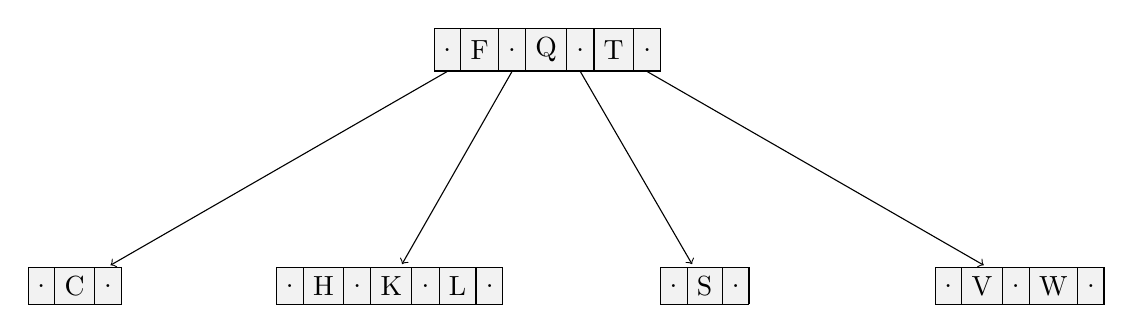
\begin{tikzpicture}[shorten >=1pt,node distance=12cm,auto]
\tikzstyle{bplus}=[rectangle split, rectangle split horizontal,rectangle split parts=#1,black,fill=gray!10,rectangle split ignore empty parts,draw]
\tikzstyle{every node}=[bplus]
\node[bplus=7](Q) at (6,3) { . \nodepart{two}  F  \nodepart{three} . \nodepart{four} Q   \nodepart{five}. \nodepart{six} T \nodepart{seven} .};
\node[bplus](C) at (0,0) { . \nodepart{two} C   \nodepart{three} .};
\node[bplus=7](K) at (4,0) {. \nodepart{two} H \nodepart{three} . \nodepart{four} K \nodepart{five} . \nodepart{six} L \nodepart{seven} .};
\node[bplus=5](S) at (8,0) {. \nodepart{two} S   \nodepart{three} .};
\node[bplus=5](V) at (12,0) {. \nodepart{two} V  \nodepart{three} . \nodepart{four} W \nodepart{five} .};


\draw[->] (Q.one south) -> (C);
\draw[->] (Q.three south) -> (K);
\draw[->] (Q.five south) -> (S);
\draw[->] (Q.seven south) -> (V);
\end{tikzpicture}
\newline
\end{center}



\item 插入M ($ [H,K,L].length \geq 2 \times t = 3  ,split [H,K,L] $)

\begin{center}
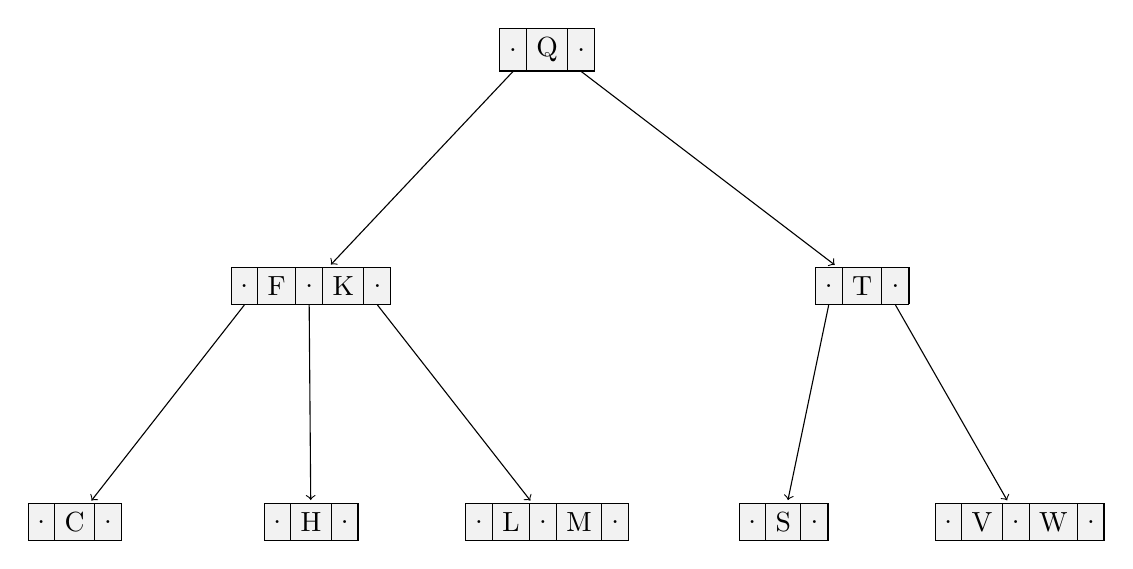
\begin{tikzpicture}[shorten >=1pt,node distance=12cm,auto]
\tikzstyle{bplus}=[rectangle split, rectangle split horizontal,rectangle split parts=#1,black,fill=gray!10,rectangle split ignore empty parts,draw]
\tikzstyle{every node}=[bplus]
\node[bplus=7](Q) at (6,6) {  . \nodepart{two} Q   \nodepart{three}.};
\node[bplus=5](F) at (3,3) { . \nodepart{two}  F  \nodepart{three} . \nodepart{four} K \nodepart{five} .}; 
\node[bplus](T) at (10,3) { . \nodepart{two}  T  \nodepart{three} .}; 
\node[bplus](C) at (0,0) { . \nodepart{two} C   \nodepart{three} .};
\node[bplus=7](H) at (3,0) {. \nodepart{two} H \nodepart{three}   .}; 
\node[bplus=5](M) at (6,0) {. \nodepart{two} L \nodepart{three} . \nodepart{four} M \nodepart{five} .}; 
\node[bplus=5](S) at (9,0) {. \nodepart{two} S   \nodepart{three} .};
\node[bplus=5](V) at (12,0) {. \nodepart{two} V  \nodepart{three} . \nodepart{four} W \nodepart{five} .};


\draw[->] (Q.one south) -> (F);
\draw[->] (Q.three south) -> (T);
\draw[->] (F.one south) -> (C);
\draw[->] (F.three south) -> (H);
\draw[->] (F.five south) -> (M);
\draw[->] (T.one south) -> (S);
\draw[->] (T.three south) -> (V);
\end{tikzpicture}
\newline
% \newpage
\end{center}


\item 插入R

\begin{center}
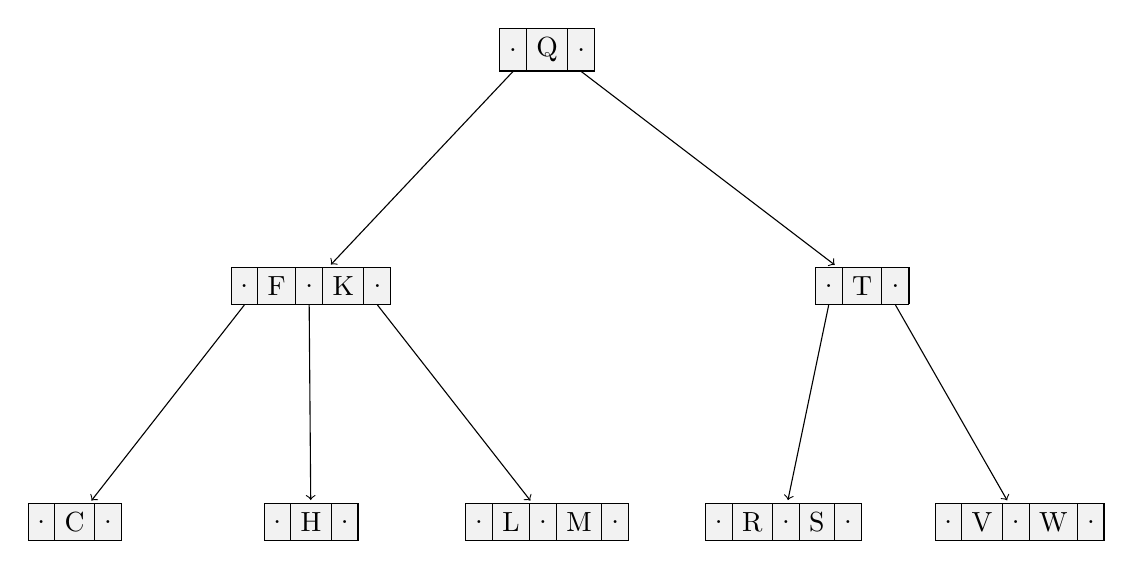
\begin{tikzpicture}[shorten >=1pt,node distance=12cm,auto]
\tikzstyle{bplus}=[rectangle split, rectangle split horizontal,rectangle split parts=#1,black,fill=gray!10,rectangle split ignore empty parts,draw]
\tikzstyle{every node}=[bplus]
\node[bplus=7](Q) at (6,6) {  . \nodepart{two} Q   \nodepart{three}.};
\node[bplus=5](F) at (3,3) { . \nodepart{two}  F  \nodepart{three} . \nodepart{four} K \nodepart{five} .}; 
\node[bplus](T) at (10,3) { . \nodepart{two}  T  \nodepart{three} .}; 
\node[bplus](C) at (0,0) { . \nodepart{two} C   \nodepart{three} .};
\node[bplus=7](H) at (3,0) {. \nodepart{two} H \nodepart{three}   .}; 
\node[bplus=5](M) at (6,0) {. \nodepart{two} L \nodepart{three} . \nodepart{four} M \nodepart{five} .}; 
\node[bplus=5](S) at (9,0) {. \nodepart{two} R   \nodepart{three}  . \nodepart{four} S \nodepart{five} .};
\node[bplus=5](V) at (12,0) {. \nodepart{two} V  \nodepart{three} . \nodepart{four} W \nodepart{five} .};


\draw[->] (Q.one south) -> (F);
\draw[->] (Q.three south) -> (T);
\draw[->] (F.one south) -> (C);
\draw[->] (F.three south) -> (H);
\draw[->] (F.five south) -> (M);
\draw[->] (T.one south) -> (S);
\draw[->] (T.three south) -> (V);
\end{tikzpicture}
\newline
\end{center}


\item 插入A

\begin{center}
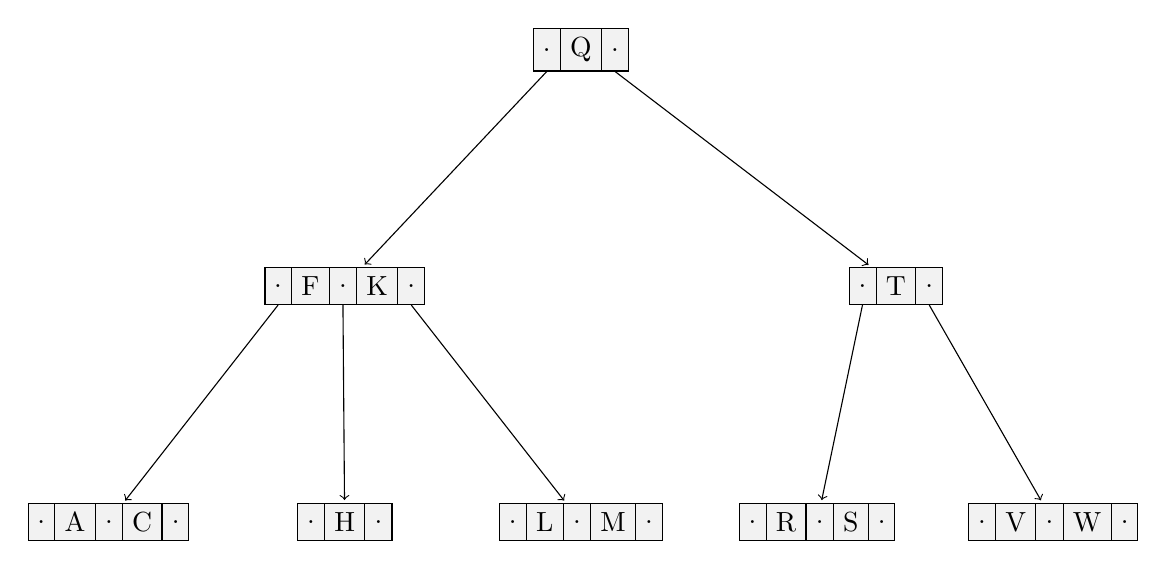
\begin{tikzpicture}[shorten >=1pt,node distance=12cm,auto]
\tikzstyle{bplus}=[rectangle split, rectangle split horizontal,rectangle split parts=#1,black,fill=gray!10,rectangle split ignore empty parts,draw]
\tikzstyle{every node}=[bplus]
\node[bplus=7](Q) at (6,6) {  . \nodepart{two} Q   \nodepart{three}.};
\node[bplus=5](F) at (3,3) { . \nodepart{two}  F  \nodepart{three} . \nodepart{four} K \nodepart{five} .}; 
\node[bplus](T) at (10,3) { . \nodepart{two}  T  \nodepart{three} .}; 
\node[bplus=5](C) at (0,0) { . \nodepart{two} A   \nodepart{three} . \nodepart{four} C \nodepart{five} .};
\node[bplus=7](H) at (3,0) {. \nodepart{two} H \nodepart{three}   .}; 
\node[bplus=5](M) at (6,0) {. \nodepart{two} L \nodepart{three} . \nodepart{four} M \nodepart{five} .}; 
\node[bplus=5](S) at (9,0) {. \nodepart{two} R   \nodepart{three}  . \nodepart{four} S \nodepart{five} .};
\node[bplus=5](V) at (12,0) {. \nodepart{two} V  \nodepart{three} . \nodepart{four} W \nodepart{five} .};


\draw[->] (Q.one south) -> (F);
\draw[->] (Q.three south) -> (T);
\draw[->] (F.one south) -> (C);
\draw[->] (F.three south) -> (H);
\draw[->] (F.five south) -> (M);
\draw[->] (T.one south) -> (S);
\draw[->] (T.three south) -> (V);
\end{tikzpicture}
\newline
% \newpage
\end{center}

\item 插入B

\begin{center}
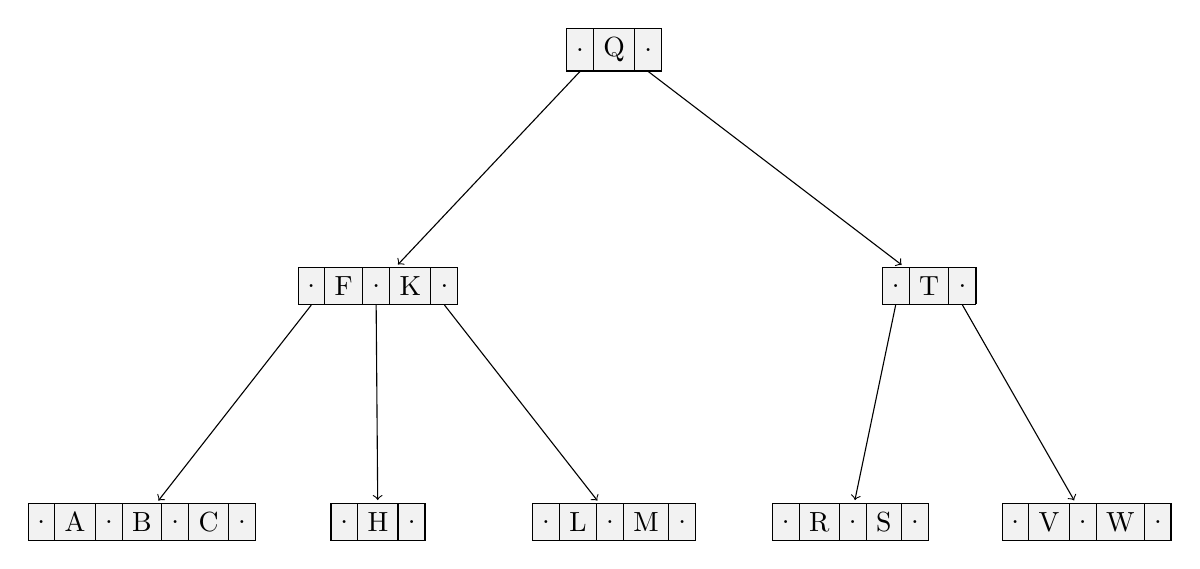
\begin{tikzpicture}[shorten >=1pt,node distance=12cm,auto]
\tikzstyle{bplus}=[rectangle split, rectangle split horizontal,rectangle split parts=#1,black,fill=gray!10,rectangle split ignore empty parts,draw]
\tikzstyle{every node}=[bplus]
\node[bplus=7](Q) at (6,6) {  . \nodepart{two} Q   \nodepart{three}.};
\node[bplus=5](F) at (3,3) { . \nodepart{two}  F  \nodepart{three} . \nodepart{four} K \nodepart{five} .}; 
\node[bplus](T) at (10,3) { . \nodepart{two}  T  \nodepart{three} .}; 
\node[bplus=7](C) at (0,0) { . \nodepart{two} A   \nodepart{three} . \nodepart{four} B \nodepart{five} . \nodepart{six} C \nodepart{seven} .};
\node[bplus=7](H) at (3,0) {. \nodepart{two} H \nodepart{three}   .}; 
\node[bplus=5](M) at (6,0) {. \nodepart{two} L \nodepart{three} . \nodepart{four} M \nodepart{five} .}; 
\node[bplus=5](S) at (9,0) {. \nodepart{two} R   \nodepart{three}  . \nodepart{four} S \nodepart{five} .};
\node[bplus=5](V) at (12,0) {. \nodepart{two} V  \nodepart{three} . \nodepart{four} W \nodepart{five} .};


\draw[->] (Q.one south) -> (F);
\draw[->] (Q.three south) -> (T);
\draw[->] (F.one south) -> (C);
\draw[->] (F.three south) -> (H);
\draw[->] (F.five south) -> (M);
\draw[->] (T.one south) -> (S);
\draw[->] (T.three south) -> (V);
\end{tikzpicture}
\newline
\end{center}


\item 插入X

\begin{center}
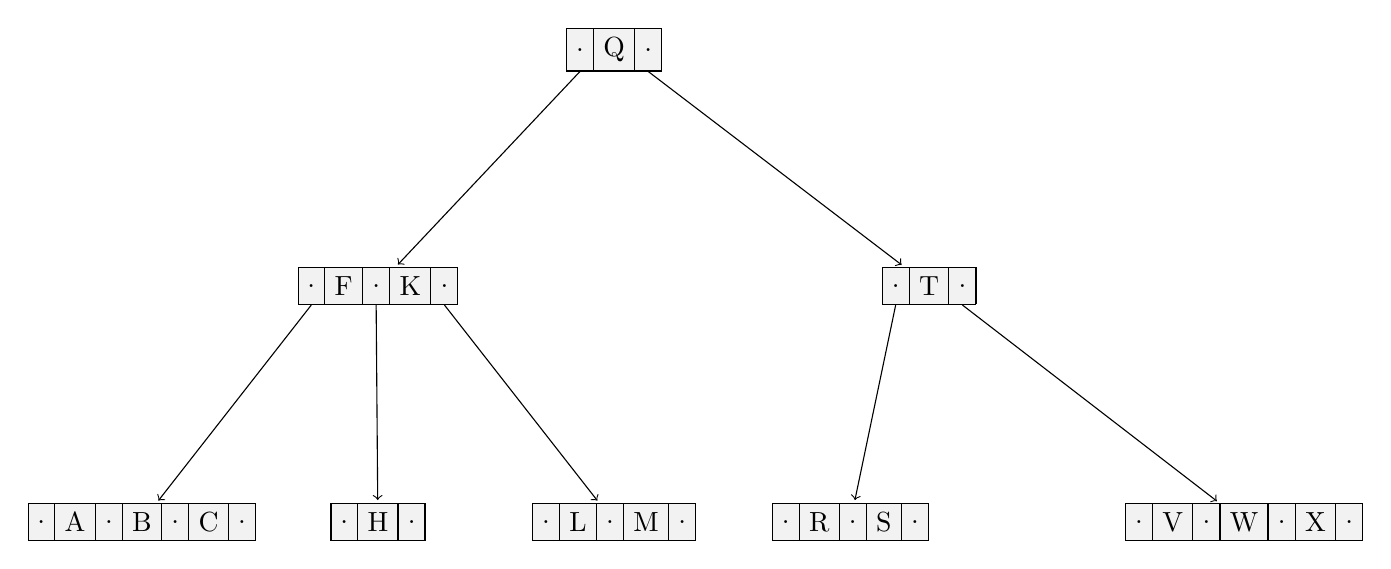
\begin{tikzpicture}[shorten >=1pt,node distance=12cm,auto]
\tikzstyle{bplus}=[rectangle split, rectangle split horizontal,rectangle split parts=#1,black,fill=gray!10,rectangle split ignore empty parts,draw]
\tikzstyle{every node}=[bplus]
\node[bplus=7](Q) at (6,6) {  . \nodepart{two} Q   \nodepart{three}.};
\node[bplus=5](F) at (3,3) { . \nodepart{two}  F  \nodepart{three} . \nodepart{four} K \nodepart{five} .}; 
\node[bplus](T) at (10,3) { . \nodepart{two}  T  \nodepart{three} .}; 
\node[bplus=7](C) at (0,0) { . \nodepart{two} A   \nodepart{three} . \nodepart{four} B \nodepart{five} . \nodepart{six} C \nodepart{seven} .};
\node[bplus=7](H) at (3,0) {. \nodepart{two} H \nodepart{three}   .}; 
\node[bplus=5](M) at (6,0) {. \nodepart{two} L \nodepart{three} . \nodepart{four} M \nodepart{five} .}; 
\node[bplus=5](S) at (9,0) {. \nodepart{two} R   \nodepart{three}  . \nodepart{four} S \nodepart{five} .};
\node[bplus=7](V) at (14,0) {. \nodepart{two} V  \nodepart{three} . \nodepart{four} W \nodepart{five} . \nodepart{six} X \nodepart{seven} .};


\draw[->] (Q.one south) -> (F);
\draw[->] (Q.three south) -> (T);
\draw[->] (F.one south) -> (C);
\draw[->] (F.three south) -> (H);
\draw[->] (F.five south) -> (M);
\draw[->] (T.one south) -> (S);
\draw[->] (T.three south) -> (V);
\end{tikzpicture}
\newline
% \newpage
\end{center}

\item 插入Y ($ [V,W,X].length \geq 2 \times t = 3  ,split [V,W,X] $)

\begin{center}
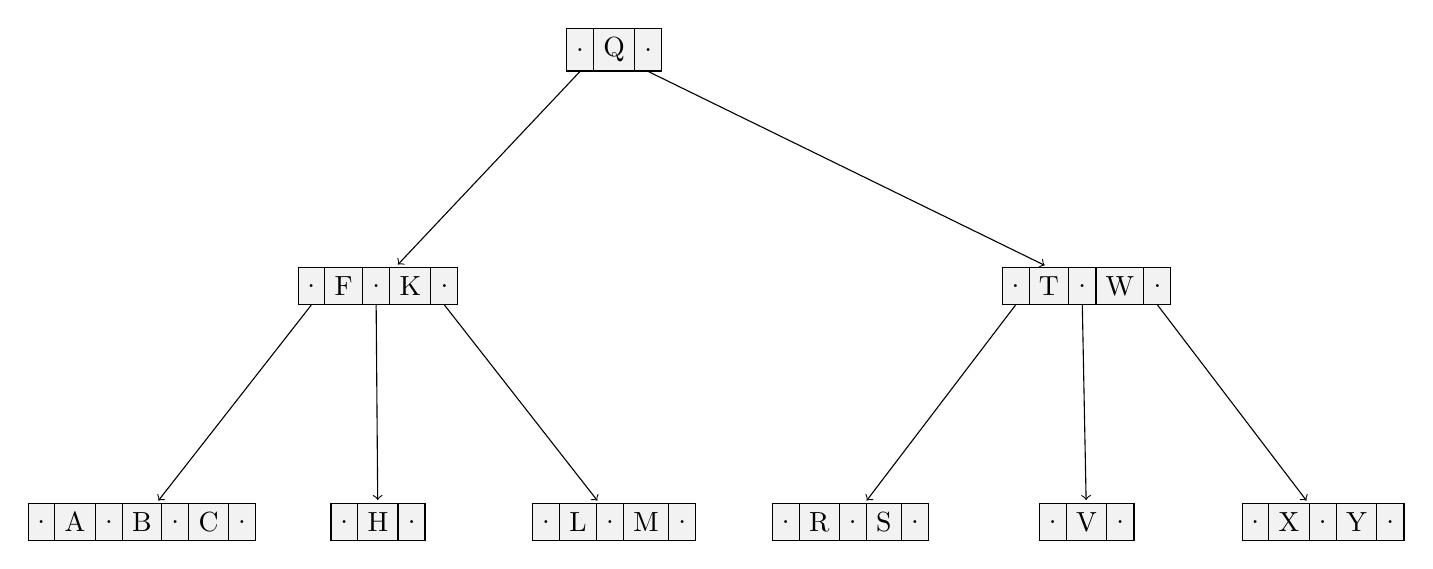
\begin{tikzpicture}[shorten >=1pt,node distance=12cm,auto]
\tikzstyle{bplus}=[rectangle split, rectangle split horizontal,rectangle split parts=#1,black,fill=gray!10,rectangle split ignore empty parts,draw]
\tikzstyle{every node}=[bplus]
\node[bplus=7](Q) at (6,6) {  . \nodepart{two} Q   \nodepart{three}.};
\node[bplus=5](F) at (3,3) { . \nodepart{two}  F  \nodepart{three} . \nodepart{four} K \nodepart{five} .}; 
\node[bplus=5](T) at (12,3) { . \nodepart{two}  T  \nodepart{three} . \nodepart{four} W \nodepart{five} .}; 
\node[bplus=7](C) at (0,0) { . \nodepart{two} A   \nodepart{three} . \nodepart{four} B \nodepart{five} . \nodepart{six} C \nodepart{seven} .};
\node[bplus=7](H) at (3,0) {. \nodepart{two} H \nodepart{three}   .}; 
\node[bplus=5](M) at (6,0) {. \nodepart{two} L \nodepart{three} . \nodepart{four} M \nodepart{five} .}; 
\node[bplus=5](S) at (9,0) {. \nodepart{two} R   \nodepart{three}  . \nodepart{four} S \nodepart{five} .};
\node[bplus=7](V) at (12,0) {. \nodepart{two} V  \nodepart{three} .}; 
\node[bplus=7](Y) at (15,0) {. \nodepart{two} X  \nodepart{three} . \nodepart{four} Y \nodepart{five} . };


\draw[->] (Q.one south) -> (F);
\draw[->] (Q.three south) -> (T);
\draw[->] (F.one south) -> (C);
\draw[->] (F.three south) -> (H);
\draw[->] (F.five south) -> (M);
\draw[->] (T.one south) -> (S);
\draw[->] (T.three south) -> (V);
\draw[->] (T.five south) -> (Y);
\end{tikzpicture}
\newline
\end{center}

\item 插入D ($ [A,B,C].length \geq 2 \times t = 3  ,split [A,B,C] $)

\begin{center}
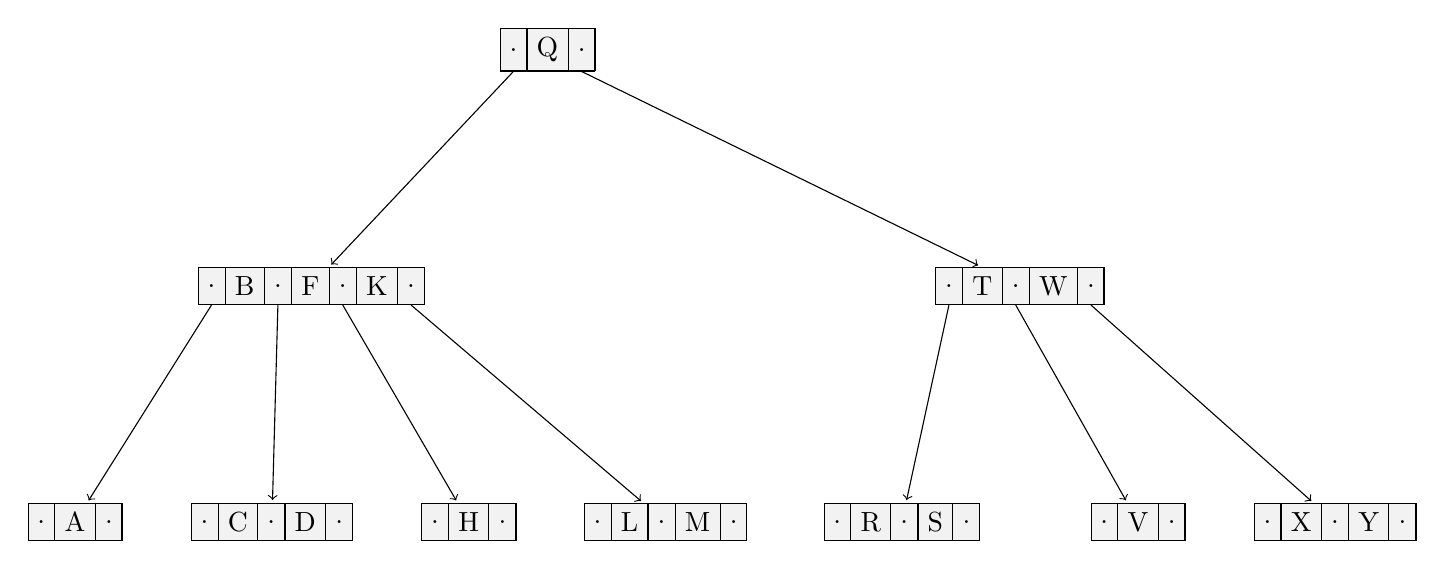
\begin{tikzpicture}[shorten >=1pt,node distance=12cm,auto]
\tikzstyle{bplus}=[rectangle split, rectangle split horizontal,rectangle split parts=#1,black,fill=gray!10,rectangle split ignore empty parts,draw]
\tikzstyle{every node}=[bplus]
\node[bplus=7](Q) at (6,6) {  . \nodepart{two} Q   \nodepart{three}.};
\node[bplus=7](F) at (3,3) { . \nodepart{two}  B  \nodepart{three} . \nodepart{four} F \nodepart{five} . \nodepart{six} K \nodepart{seven} .}; 
\node[bplus=5](T) at (12,3) { . \nodepart{two}  T  \nodepart{three} . \nodepart{four} W \nodepart{five} .}; 
\node[bplus=7](A) at (0,0) { . \nodepart{two} A   \nodepart{three} . };
\node[bplus=7](C) at (2.5,0) { . \nodepart{two} C   \nodepart{three} .  \nodepart{four} D \nodepart{five} .};
\node[bplus=7](H) at (5,0) {. \nodepart{two} H \nodepart{three}   .}; 
\node[bplus=5](M) at (7.5,0) {. \nodepart{two} L \nodepart{three} . \nodepart{four} M \nodepart{five} .}; 
\node[bplus=5](S) at (10.5,0) {. \nodepart{two} R   \nodepart{three}  . \nodepart{four} S \nodepart{five} .};
\node[bplus=7](V) at (13.5,0) {. \nodepart{two} V  \nodepart{three} .}; 
\node[bplus=7](Y) at (16,0) {. \nodepart{two} X  \nodepart{three} . \nodepart{four} Y \nodepart{five} . };


\draw[->] (Q.one south) -> (F);
\draw[->] (Q.three south) -> (T);
\draw[->] (F.one south) -> (A);
\draw[->] (F.three south) -> (C);
\draw[->] (F.five south) -> (H);
\draw[->] (F.seven south) -> (M);
\draw[->] (T.one south) -> (S);
\draw[->] (T.three south) -> (V);
\draw[->] (T.five south) -> (Y);
\end{tikzpicture}
\newline
% \newpage
\end{center}

\item 插入Z

\begin{center}
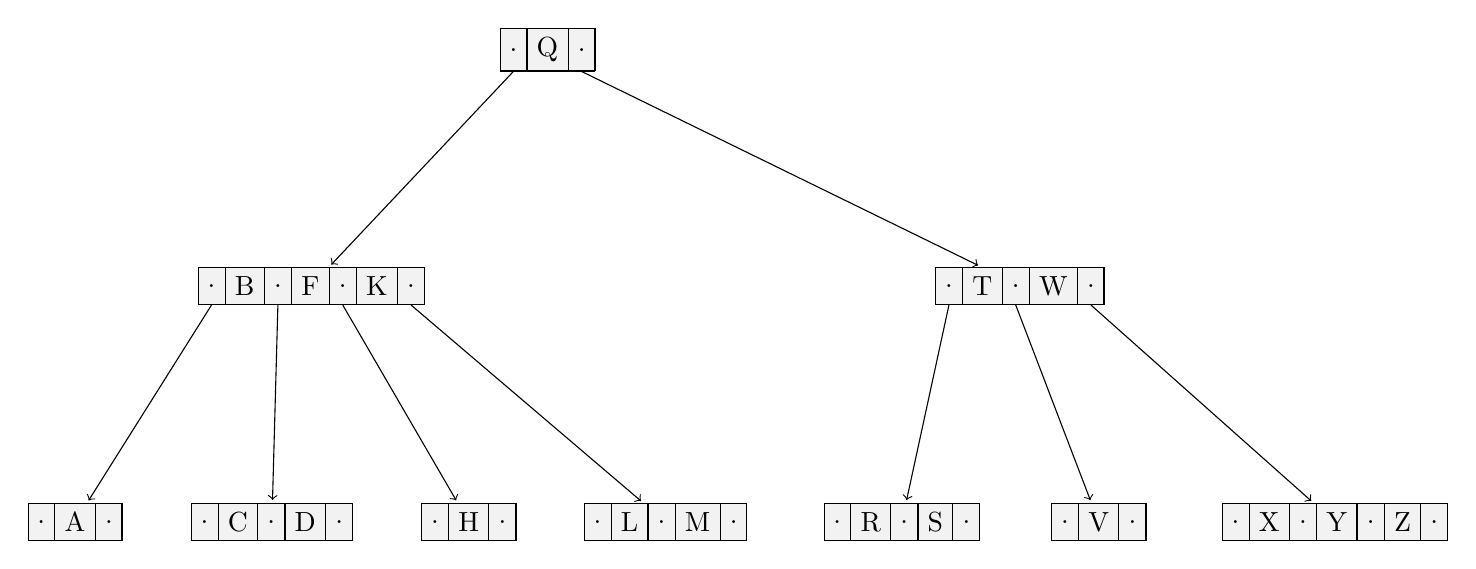
\begin{tikzpicture}[shorten >=1pt,node distance=12cm,auto]
\tikzstyle{bplus}=[rectangle split, rectangle split horizontal,rectangle split parts=#1,black,fill=gray!10,rectangle split ignore empty parts,draw]
\tikzstyle{every node}=[bplus]
\node[bplus=7](Q) at (6,6) {  . \nodepart{two} Q   \nodepart{three}. };
\node[bplus=7](F) at (3,3) { . \nodepart{two}  B  \nodepart{three} . \nodepart{four} F \nodepart{five} . \nodepart{six} K \nodepart{seven} .}; 
\node[bplus=5](T) at (12,3) { . \nodepart{two}  T  \nodepart{three} . \nodepart{four} W \nodepart{five} .}; 
\node[bplus=7](A) at (0,0) { . \nodepart{two} A   \nodepart{three} . };
\node[bplus=7](C) at (2.5,0) { . \nodepart{two} C   \nodepart{three} .  \nodepart{four} D \nodepart{five} .};
\node[bplus=7](H) at (5,0) {. \nodepart{two} H \nodepart{three}   .}; 
\node[bplus=5](M) at (7.5,0) {. \nodepart{two} L \nodepart{three} . \nodepart{four} M \nodepart{five} .}; 
\node[bplus=5](S) at (10.5,0) {. \nodepart{two} R   \nodepart{three}  . \nodepart{four} S \nodepart{five} .};
\node[bplus=7](V) at (13,0) {. \nodepart{two} V  \nodepart{three} .}; 
\node[bplus=7](Y) at (16,0) {. \nodepart{two} X  \nodepart{three} . \nodepart{four} Y \nodepart{five} . \nodepart{six} Z \nodepart{seven} .};


\draw[->] (Q.one south) -> (F);
\draw[->] (Q.three south) -> (T);
\draw[->] (F.one south) -> (A);
\draw[->] (F.three south) -> (C);
\draw[->] (F.five south) -> (H);
\draw[->] (F.seven south) -> (M);
\draw[->] (T.one south) -> (S);
\draw[->] (T.three south) -> (V);
\draw[->] (T.five south) -> (Y);
\end{tikzpicture}
\newline
\end{center}

\item 插入E

\begin{center}
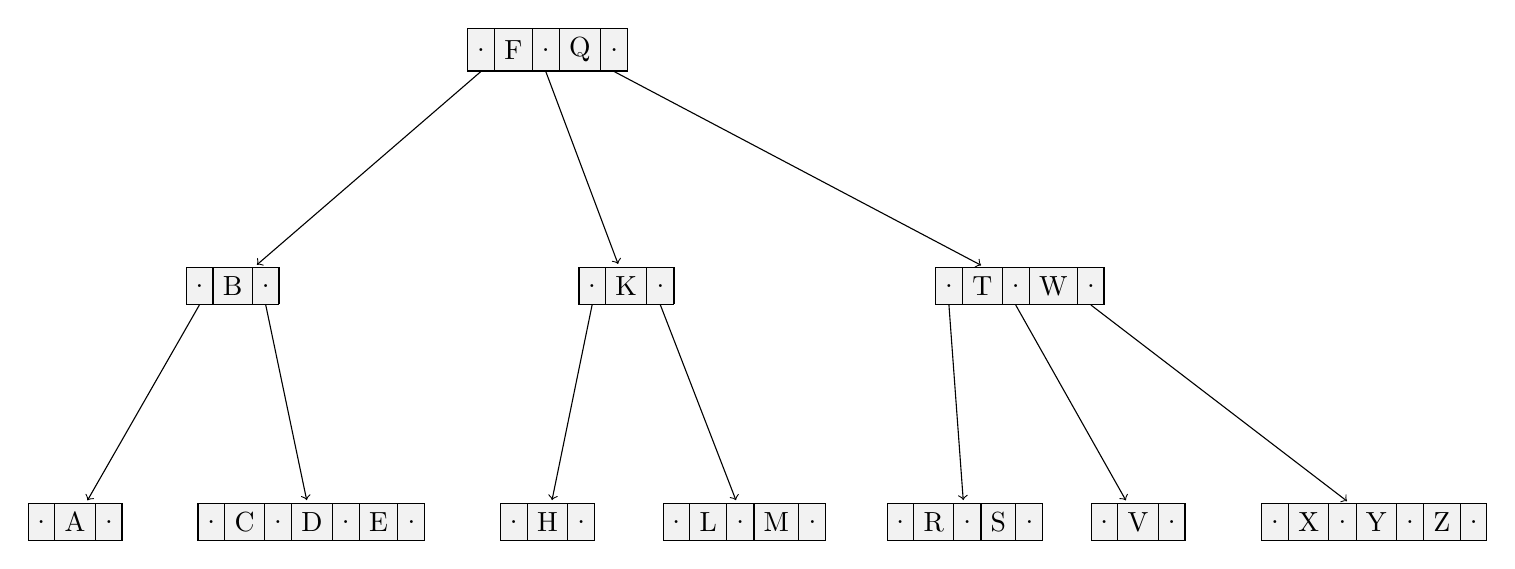
\begin{tikzpicture}[shorten >=1pt,node distance=12cm,auto]
\tikzstyle{bplus}=[rectangle split, rectangle split horizontal,rectangle split parts=#1,black,fill=gray!10,rectangle split ignore empty parts,draw]
\tikzstyle{every node}=[bplus]
\node[bplus=7](Q) at (6,6) {  . \nodepart{two} F   \nodepart{three}. \nodepart{four} Q \nodepart{five} .};
\node[bplus=7](B) at (2,3) { . \nodepart{two}  B  \nodepart{three} . };
\node[bplus=7](K) at (7,3) { . \nodepart{two}  K  \nodepart{three} . };
\node[bplus=5](T) at (12,3) { . \nodepart{two}  T  \nodepart{three} . \nodepart{four} W \nodepart{five} .}; 
\node[bplus=7](A) at (0,0) { . \nodepart{two} A   \nodepart{three} . };
\node[bplus=7](C) at (3,0) { . \nodepart{two} C   \nodepart{three} .  \nodepart{four} D \nodepart{five} . \nodepart{six} E \nodepart{seven} .};
\node[bplus=7](H) at (6,0) {. \nodepart{two} H \nodepart{three}   .}; 
\node[bplus=5](M) at (8.5,0) {. \nodepart{two} L \nodepart{three} . \nodepart{four} M \nodepart{five} .}; 
\node[bplus=5](S) at (11.3,0) {. \nodepart{two} R   \nodepart{three}  . \nodepart{four} S \nodepart{five} .};
\node[bplus=7](V) at (13.5,0) {. \nodepart{two} V  \nodepart{three} .}; 
\node[bplus=7](Y) at (16.5,0) {. \nodepart{two} X  \nodepart{three} . \nodepart{four} Y \nodepart{five} . \nodepart{six} Z \nodepart{seven} .};


\draw[->] (Q.one south) -> (B);
\draw[->] (Q.three south) -> (K);
\draw[->] (Q.five south) -> (T);
\draw[->] (B.one south) -> (A);
\draw[->] (B.three south) -> (C);
\draw[->] (K.one south) -> (H);
\draw[->] (K.three south) -> (M);
\draw[->] (T.one south) -> (S);
\draw[->] (T.three south) -> (V);
\draw[->] (T.five south) -> (Y);
\end{tikzpicture}
\newline
\end{center}

\end{enumerate}
\end{large}
\end{document}
